\chapter{Analisi e progettazione}
\label{cha:analisi_progettazione}
Da una prima analisi dei prodotti esistenti per i trasporti pubblici, in particolare della Provincia Autonoma di Trento, è emerso che non esiste un'unica applicazione che racchiuda tutte le informazioni utili per i viaggiatori. Come visto nel capitolo precedente, esistono diverse applicazioni per gli orari in tempo reale e la ricerca dei percorsi a livello provinciale; mentre, per i servizi nazionali è necessario utilizzare ulteriori applicazioni o siti web (\textit{ViaggiaTreno, Trenitalia.it}).
Per questo motivo ho deciso di implementare un applicativo che racchiuda tutte queste informazioni in maniera semplice ed intuitiva. 
Le tre possibilità per l'implementazione sono: un'applicazione mobile, un sito web e un chatbot. Dopo un'attenta valutazione delle opzioni, ho deciso di creare un bot Telegram, vista la possibilità di utilizzarlo su tutti i sistemi operativi in maniera agevole.  

\section{Perché un bot di Telegram?}

\begin{wrapfigure}{r}{0.33\textwidth}
\centering

\includegraphics[width=5.5cm]{telegram-logo.png}
\caption{Telegram logo}
\label{fig:telegram_logo}
\end{wrapfigure}

Telegram è un'app di messaggistica mobile e desktop basata sul cloud, focalizzata su sicurezza e velocità. \cite{Telegram} Oltre a ciò, offre altre funzionalità, come i canali, con lo sopo di diffondere messaggi ad un ampio pubblico; e i bot, applicazioni di terze parti con cui gli utenti possono interagire inviando dei messaggi, comandi o con delle apposite tastiere. I bot consentono, ad esempio, di ricevere notifiche e news personalizzate, interagire con altri servizi, costruire giochi single- e multi-player, creare dei piccoli "social network", gestire la moderazione di gruppi e inviare automaticamente dei messaggi nei canali. 
Telegram è utilizzato da una vasta utenza, circa 1 miliardo di utenti, ed è disponibile sia su dispositivi mobile che desktop, questo permette al bot di raggiungere velocemente un ampio numero di utenti. 

\subsection{Come interagire con un bot}
Chiunque possieda un profilo Telegram può interagire con un bot con tre diverse modalità:
\begin{itemize}
\item inviare messaggi e comandi aprendo una chat privata con il bot;
\item attraverso le \textit{inline queries} (figura \ref{fig:telegram_interactions}\subref{fig:inline_queries}), l'utente può chiamare il bot scrivendo il suo username e una query nella casella di testo di qualsiasi chat. In questo modo è possibile richiedere al bot del contenuto da qualsiasi chat, gruppo o canale senza inviare alcun messaggio;
\item tramite le apposite tastiere che si suddividono in: 
\begin{itemize}
\item tastiera inline (figura \ref{fig:telegram_interactions}\subref{fig:inline_keyboard}): permette di allegare dei pulsanti direttamente ad un messaggio, l'utente premendo uno di questi genererà un azione che sarà poi gestita dal codice del bot; 
\item tastiera normale (figura \ref{fig:telegram_interactions}\subref{fig:normal_keyboard}): è formata da una serie di pulsanti nella metà inferiore della chat, al posto della tradizionale tastiera QUERTY. I bottoni, che contengono un testo, permetteranno di inviarlo al bot. 
\end{itemize}
\end{itemize}

\begin{figure}[htb]
    \centering 
\begin{subfigure}{0.25\textwidth}
\frame{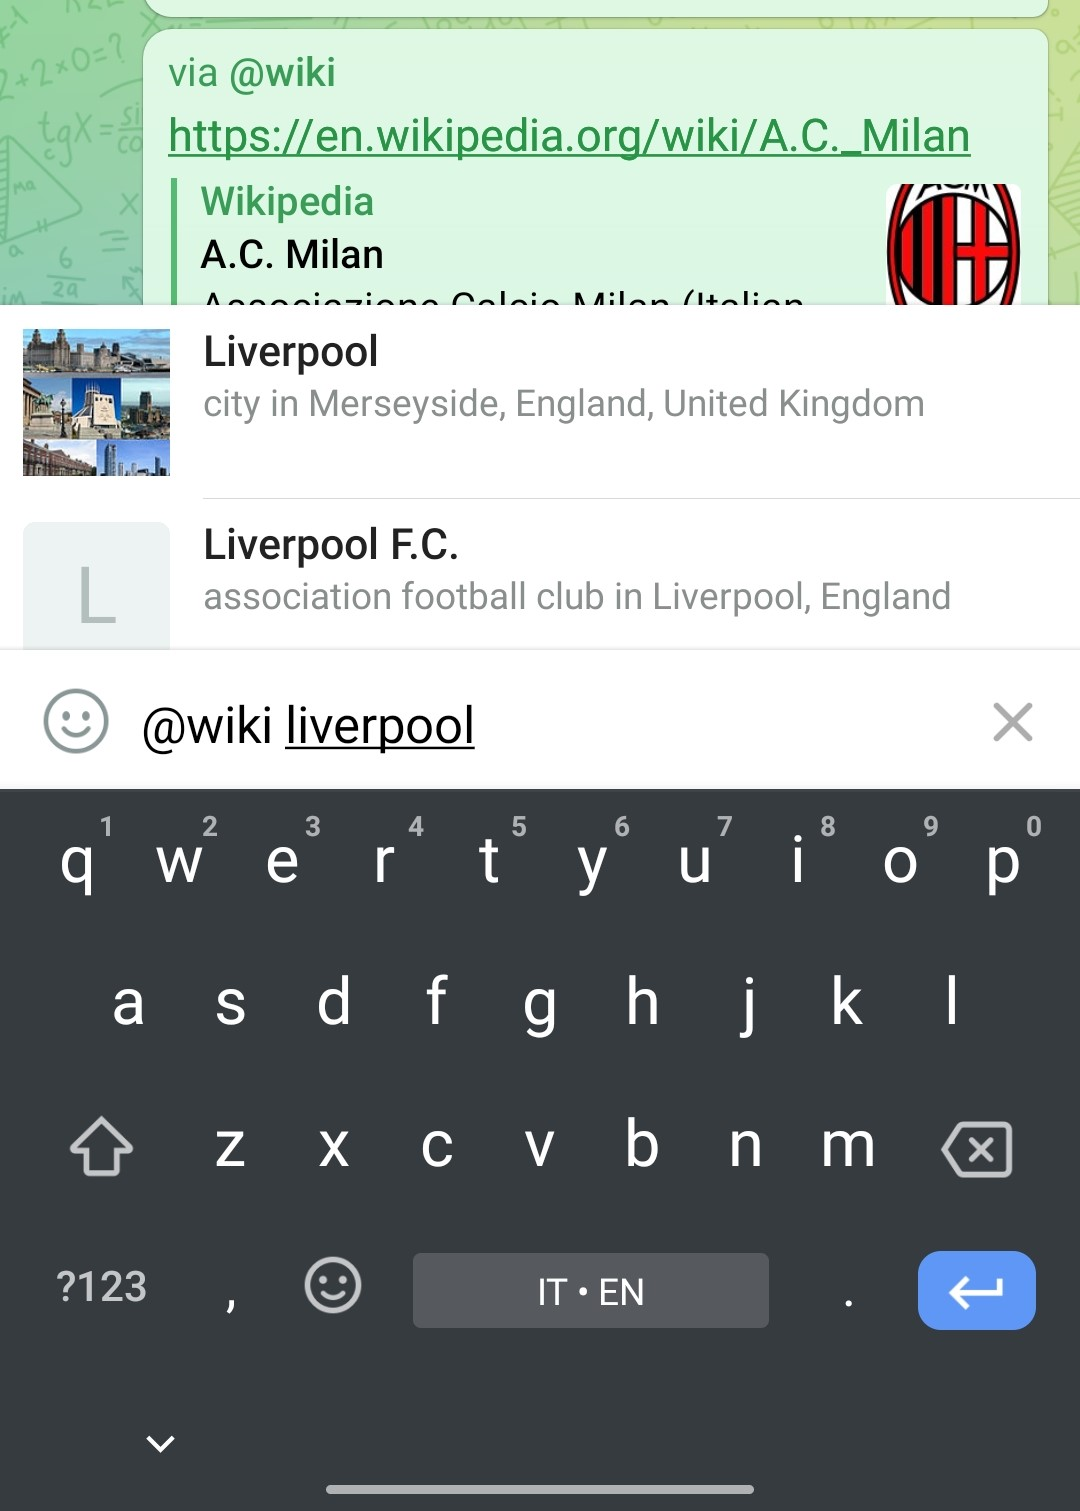
\includegraphics[width=\linewidth]{inline_queries.jpg}}
\caption{Inline queries}
\label{fig:inline_queries}
\end{subfigure}\hfil
\begin{subfigure}{0.25\textwidth}
\frame{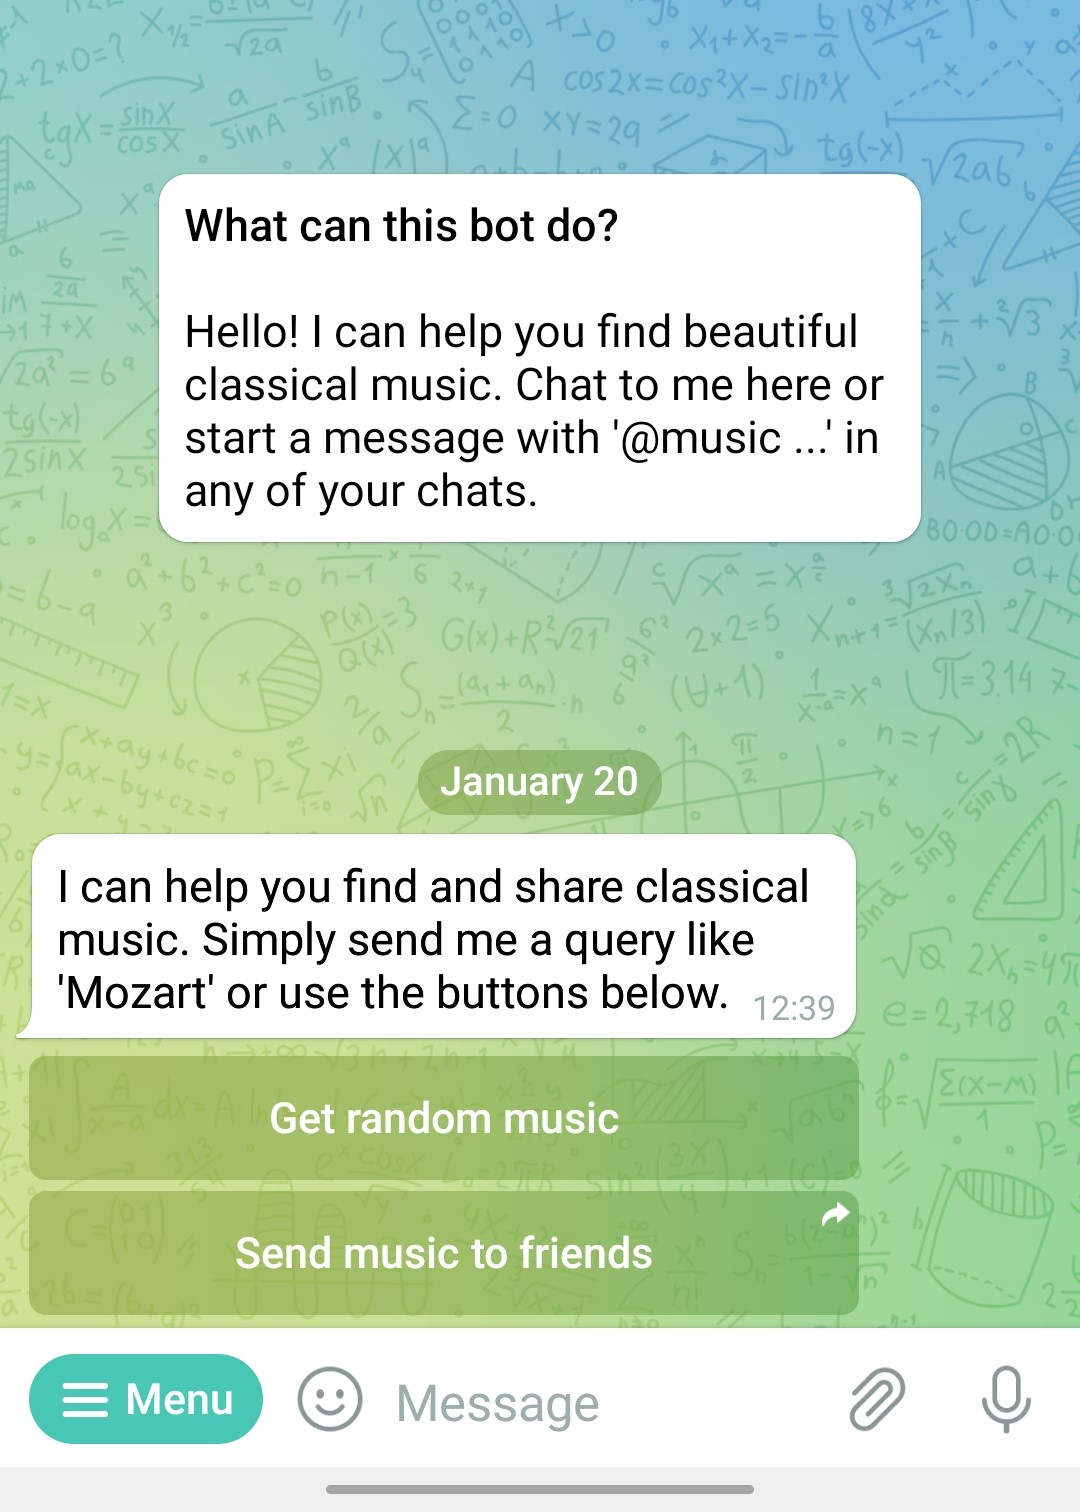
\includegraphics[width=\linewidth]{tastiera_inline.jpg}}
\caption{Tastiera inline}
\label{fig:inline_keyboard}
\end{subfigure}\hfil 
\begin{subfigure}{0.25\textwidth}
\frame{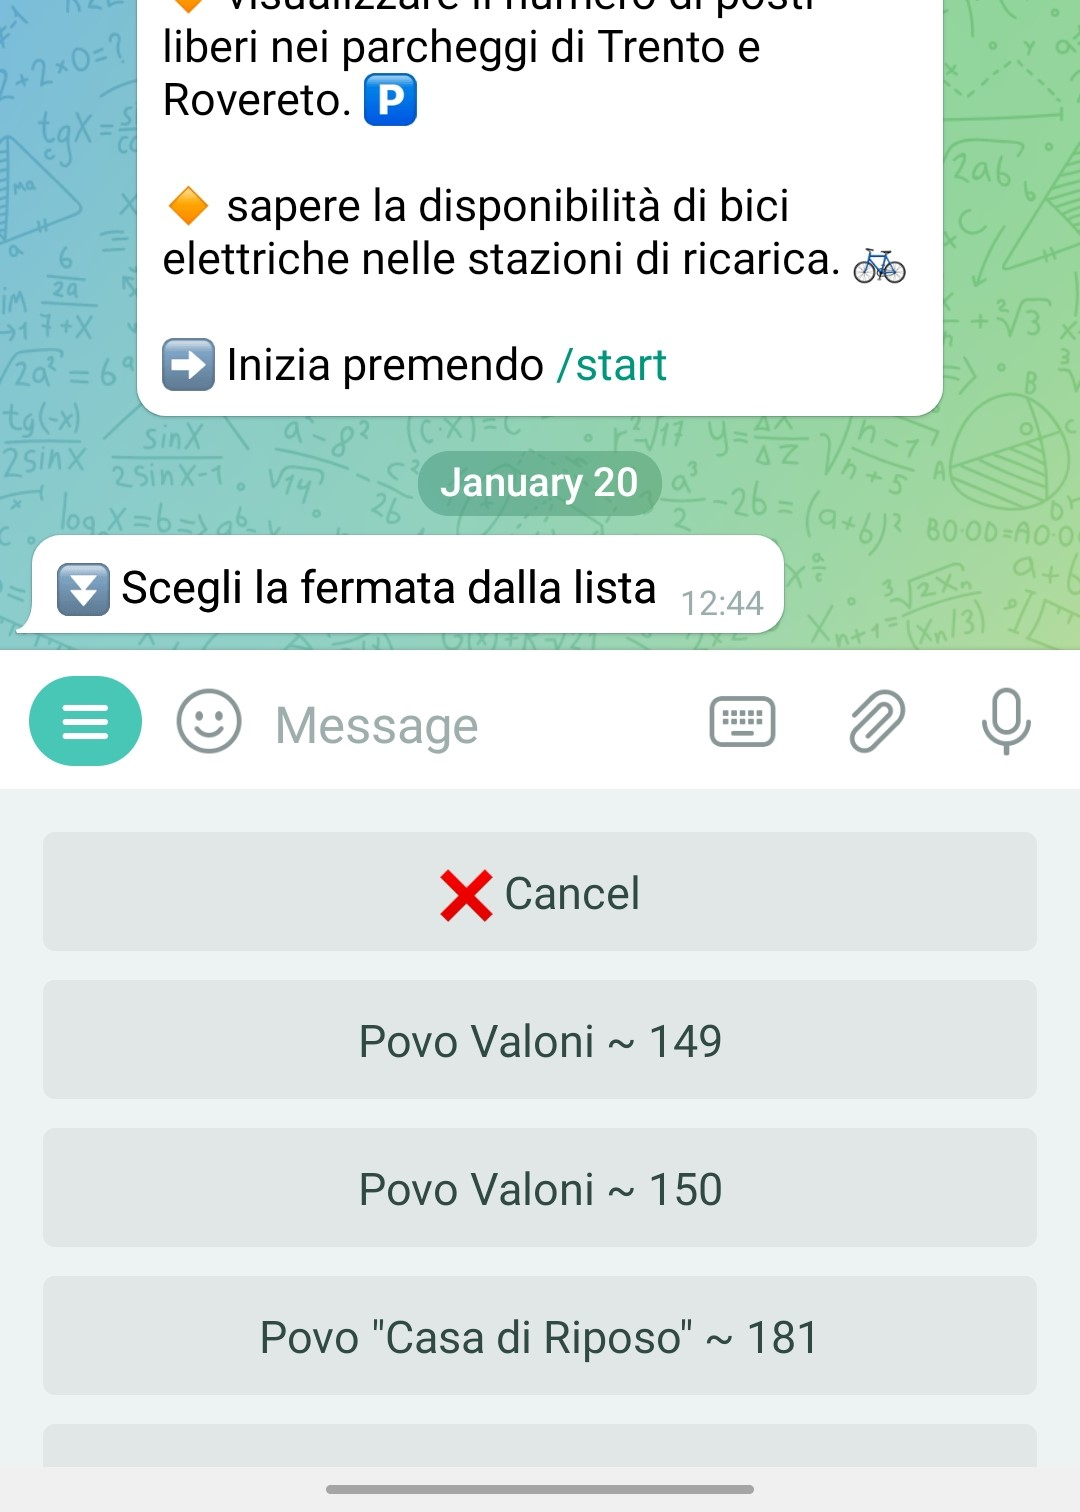
\includegraphics[width=\linewidth]{tastiera_normale.jpg}}
\caption{Tastiera normale}
\label{fig:normal_keyboard}
\end{subfigure}

\caption{
\label{fig:telegram_interactions}Interazioni Telegram bot}
\end{figure}

\pagebreak

\section{Analisi dei requisiti}
\label{sec:requisiti}

Come descritto in precedenza lo scopo principale di questo bot è raccogliere in unico applicativo varie informazioni sui trasporti pubblici della Provincia di Trento. 
In particolare si vuole dare la possibilità agli utenti di:
\begin{itemize}
\item consultare gli orari di autobus urbani e extraurbani;
\item consultare gli orari delle ferrovie Brennero, Valsugana e Trento-Mezzana;
\item visualizzare su una mappa dove si trova un autobus in tempo reale e avere la possibilità di seguirlo durante il suo percorso;
\item visualizzare il ritardo e l'ultima posizione conosciuta dei mezzi;
\item visualizzare il numero di posti liberi nei parcheggi dei comuni di Trento e Rovereto;
\item sapere la disponibilità di bici presenti nelle stazioni del bike sharing;
\item salvare le fermate e linee preferite per una consultazione di orari e ritardi molto più veloce;
\item rimanere informati su eventuali scioperi, variazioni di percorso, fermate sospese.
\end{itemize}

Alcuni requisiti, come l'acquisto dei biglietti e la ricerca dei singoli percorsi, sono stati esclusi da questa prima versione. In particolare, il primo per difficoltà nella vendita dei biglietti, data la mancanza di API pubbliche apposite; mentre il secondo ha ricevuto una priorità minore. 

\section{Progettazione}
\label{sec:progettazione}

Il prodotto, in questo caso il Bot, deve essere progettato intorno alle persone. Quindi, per avere una più chiara visione dei comportamenti, abitudini e bisogni del nostro target di riferimento ho deciso di creare 2 personas e 2 scenari.

I \textit{personas} sono personaggi di fantasia che rappresentano un possibile gruppo di utenti reali. Mentre, gli \textit{scenari} consistono in una ricostruzione dettagliata di una situazione d'utilizzo. 

\subsection{Personas}
\begin{itemize}
\item \textbf{Antonio} è uno studente universitario pendolare di 21 anni, abita a Rovereto e, quindi, utilizza il treno e i bus di linea per andare all'università, in biblioteca o in mensa. Ogni mattina, per controllare gli orari e i ritardi del treno regionale e del bus, ha bisogno di consultare più applicazioni. Gli piacerebbe, quindi, avere un unico applicativo per poter controllare tutti le informazioni necessarie.
\item \textbf{Francesca} è una turista di 35 anni, è arrivata in Trentino in treno. Durante la sua permanenza ha deciso di utilizzare solo i mezzi pubblici e le bici elettriche in sharing per raggiungere i vari luoghi di interesse. Ha molta dimestichezza con i dispositivi digitali, la sua esigenza chiave è poter visitare più destinazioni possibili e non perdere tempo inutilmente.  
\end{itemize}

\subsection{Scenari}
\begin{itemize}
\item \textbf{Scenario A}: l'utente è alla fermata dell'autobus e sono già passati 5 minuti dall'orario previsto di arrivo, decide allora di controllare sul bot Telegram il ritardo accumulato. Una volta scoperto che il ritardo previsto eri di ulteriori 15 minuti, decide di andare a bere un caffè. 

\begin{figure}[h]
\centering
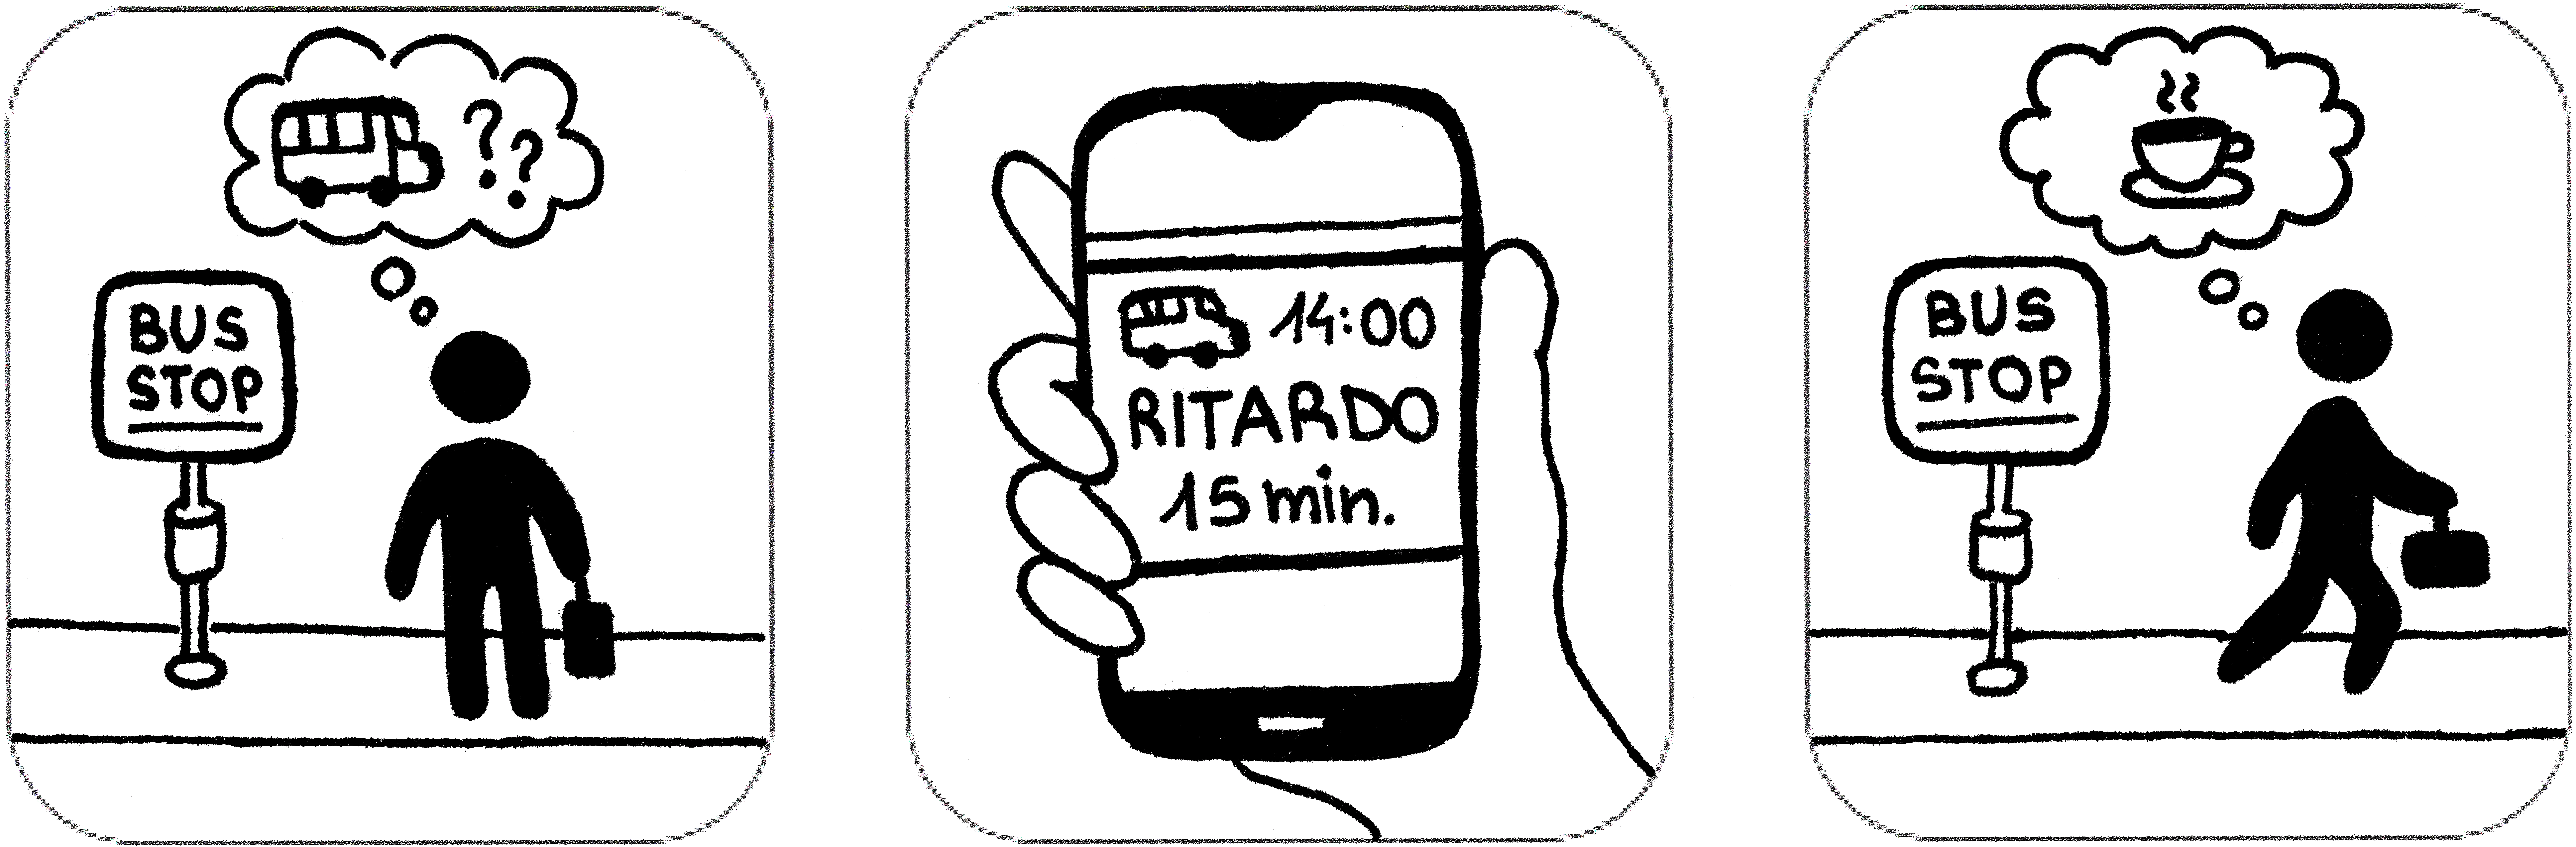
\includegraphics[width=0.9\textwidth]{scenario_1.png}
\caption{Scenario A}
\label{fig:scenarios_A}
\end{figure}

\item \textbf{Scenario B}: l'utente vuole prendere una bici elettrica in sharing, una volta arrivato alla stazione di ricarica non ne trova nessuna disponibile. Controlla allora sul bot qual è la stazione più vicina alla sua posizione attuale dove poter trovare una bici. 

\begin{figure}[h]
\centering
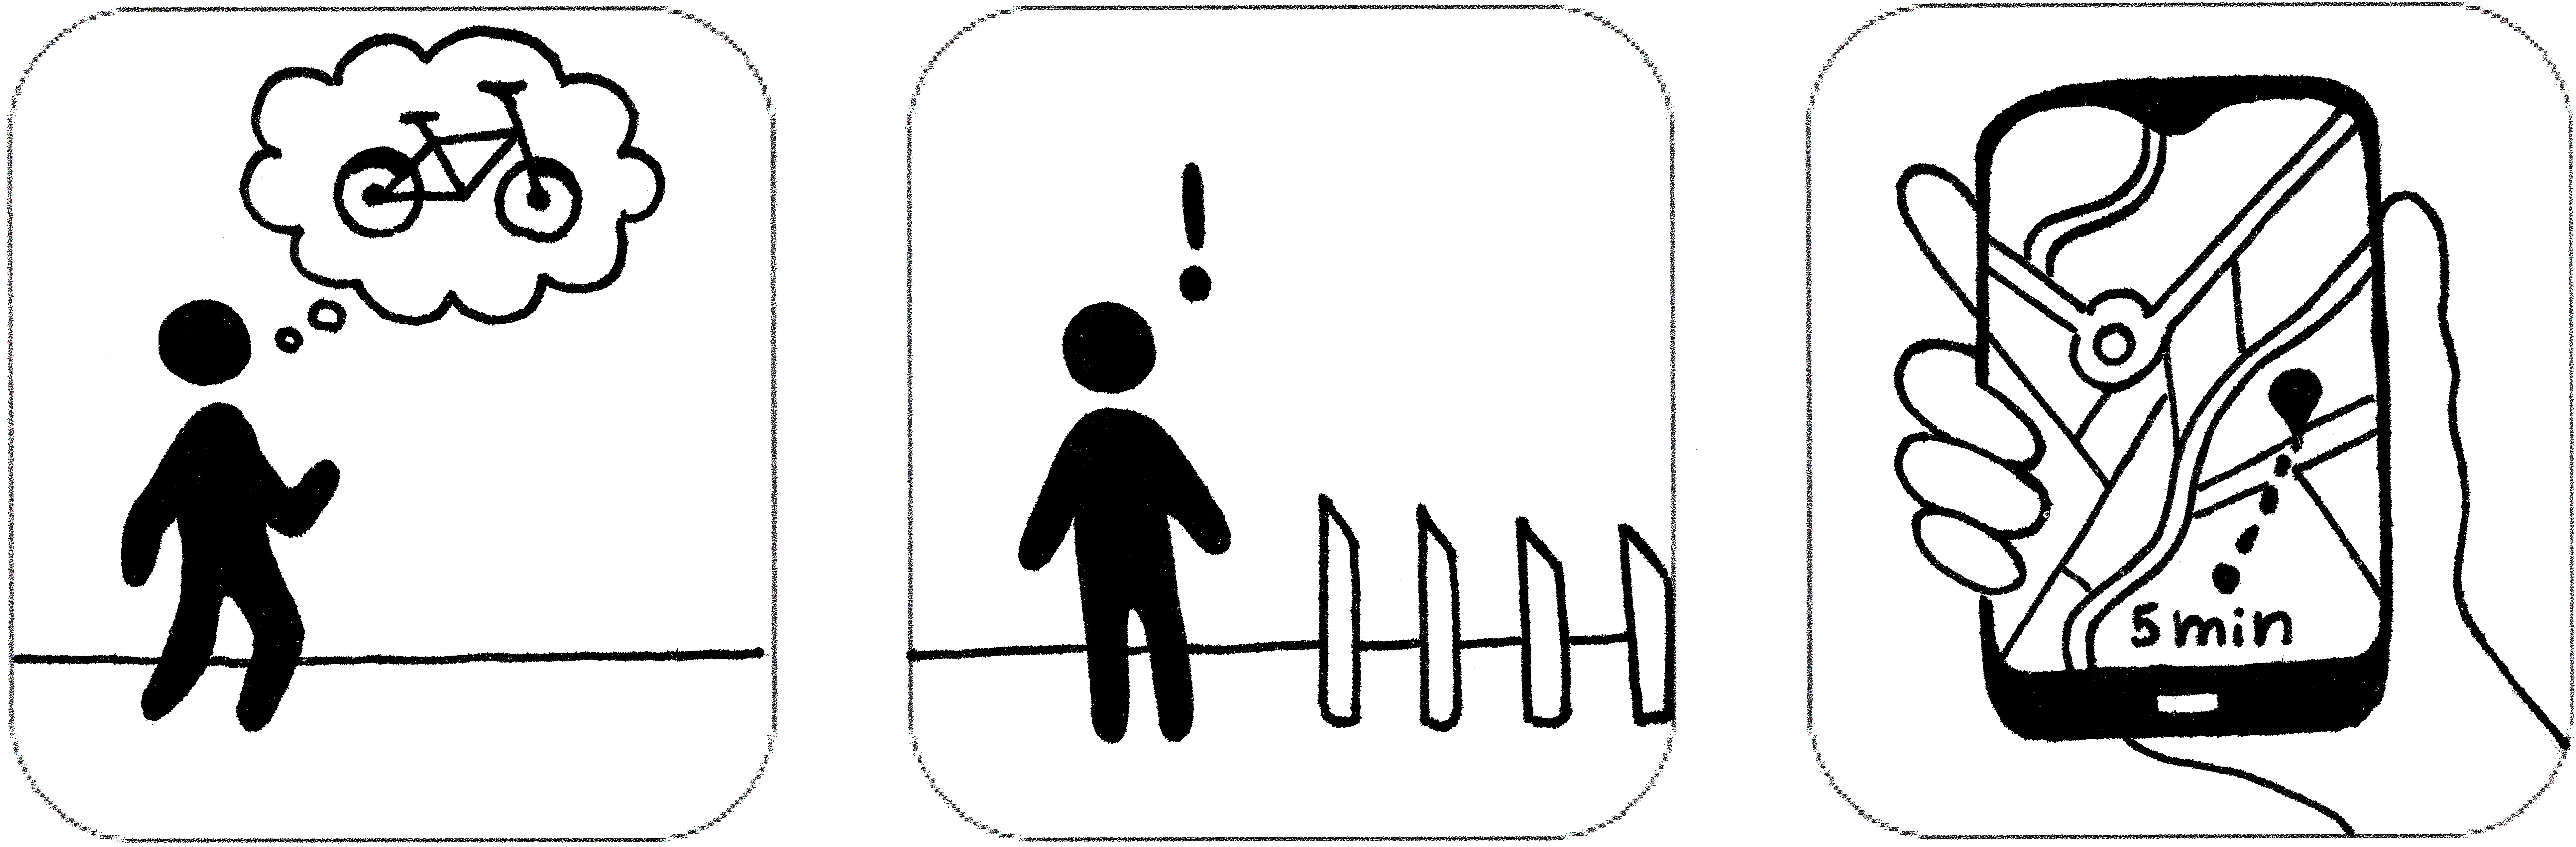
\includegraphics[width=0.9\textwidth]{scenario_2.png}
\caption{Scenario B}
\label{fig:scenarios_B}
\end{figure}

\end{itemize}

\subsection{Servizi esterni}

Per fornire dati reali e utili è stato necessario avvalersi di vari servizi esterni. In particolare: 
\begin{itemize}
\item gli orari e le informazioni sulle fermate degli autobus urbani ed extra urbani sono forniti in formato CSV dal sito \textit{opendata} di Trentino Trasporti \cite{opendataTrentinoTrasporti}
\item le informazioni in tempo reale provengono dalle API dell'applicazione \textit{Muoversi in Trentino}
\item gli orari dei treni sono fornite dalle API del servizio \textit{ViaggiaTreno}
\item i dati sui parcheggi e sulle stazioni di ricarica delle biciclette provengono dalle API delle applicazioni mobile \textit{ViaggiaTrento} e \textit{ViaggiaRovereto}.
\end{itemize}

\subsection{Struttura e interfaccia del bot}
Il bot è stato pensato per funzionare sia utilizzando la tastiera inline che i comandi. 
L'interfaccia con cui ci troveremo ad interagire presenterà una serie di pulsanti inline con i quali sarà possibile navigare tra le diverse funzioni. Le informazioni saranno inviate prevalentemente tramite messaggi testuali arricchiti da emoji utili a rende l'esperienza dell'utente più dinamica e comprensibile. 
Un'ulteriore funzionalità sarà la possibilità di osservare su una mappa, in tempo reale, l'ultima posizione rilevata di un autobus e per fare ciò verrà utilizzata la funzione di \textit{live location} fornita da Telegram. 
Le news su eventuali scioperi, variazioni di percorso, fermate sospese, invece, verranno inviate automaticamente dal bot su un canale Telegram dedicato. 

\subsection{Database}
Il bot avrà bisogno di un database in cloud per gestire le preferenze degli utenti, come fermate e linee preferite, e le sessioni di questi. In particolare, si dovranno gestire le sessioni in quanto i messaggi di Telegram sono inviati in maniera indipendente uno dall'altro. Risulta quindi necessario un meccanismo per gestire scenari complessi in cui un'azione dipende da una precedente. 

\newpage